\chapter{Data Streams} 
\label{chap:data_stream_processing}
With the advent of the \emph{Big Data} era, large amounts of data are being generated 
by companies from their infrastructure; from IoT sensors to events 
generated by customers using online services.
The generated data 
are \emph{unbounded} and infinite by nature, since 
new data will be generated continuously. 

For example, the healthcare industry has also been transitioning to 
adopt the approach of data-driven diagnostics methods~\cite{hospital_diagnosis}. 
This transition is caused by the need to keep up with the increase in the amount 
of physiological data generated by the monitoring sensors attached to
patients~\cite{hospital_data_monitoring}. These physiological data are usually generated 
periodically at regular intervals
in a streaming manner. 

As a consequence of the large volume and continuous data generation, there is a need for 
companies to be able to process these unbounded data streams.
Data Stream Management Systems (DSMS)
 are equipped to handle such unbounded data and are adopted 
widely in the industry today in the form of various frameworks such as Apache Flink~\cite{flink} and 
Apache Spark streaming~\cite{spark_streaming}.
The main features of these DSMSs are their ability to 
\renewcommand{\labelenumi}{(\roman{enumi})}
\begin{enumerate*}
    \item scale horizontally, 
    \item process records individually as they arrive, and
    \item process or analyse the data in real time.
\end{enumerate*}

In Chapter~\ref{chap:data_stream_processing}, we will dive into details of 
the characteristics of data streams, how a DSMS typically handles fault tolerance, and
the general strategy of processing streaming data. Finally, we will also elaborate on the 
various state-of-the-art frameworks in use by industries.
\gh{There are a lot more used in industry than Flink, Storm and Spark. See
for instance}
\url{https://en.wikipedia.org/wiki/Data_stream_management_system#Examples},
\url{https://en.wikipedia.org/wiki/Complex_event_processing#Vendors_and_products}.
\gh{Maybe, in the introduction of 3.4 list a few more of these before your motivation to describe the ones you picked.}

\section{Characteristics of Data Streams}
\label{sec:characteristics_data_stream}
What is a data stream? As defined by Golab and Ozsu~\cite{golab_data_stream}:
“A \emph{data stream} is a \emph{real-time}, continuous, ordered (implicitly by arrival time 
or explicitly by timestamp) sequence of items. It is impossible to control the order
in which items arrive, nor is it feasible to \emph{locally store} a stream in its entirety.”
The difference between traditional Big Data processing and data stream processing, lies in 
the inability to store the whole dataset \emph{locally} for data streams management. Furthermore, 
the use cases of data stream processing require realtime responses with low latency.

Big Data is usually characterized with the three “V's: \emph{volume}, \emph{velocity} 
and \emph{variety}~\cite{big_data_analytics}.
In the context of data streams processing, it is expected that the \emph{volume} of 
the data is unbounded since the devices, sensors and applications are constantly 
generating data as long as there is an uptime. The \emph{variety} aspect of the 
data streams is also heterogeneous in nature where different sources used by the same 
processing engine may emit different types of data; structured and unstructured. 
Moreover, \emph{variety} in data can also happen over time; a concept drift where 
the properties of data may change over time unlike Big Data. 

Out of the three aforementioned characteristics, \emph{velocity} is the most important 
factor to consider when it comes to data stream processing. Data in a streaming 
environment is rapidly changing, and they arrive constantly into the stream processing
pipeline and needs to be processed within a limited time frame.
As a result, it is infeasible to have random memory access capability
over the entire stream
 --- only single pass algorithms can
be applied. This requirement of low latency processing has the consequence 
that late decisions will result in missed opportunities. Related to \emph{velocity}, 
the data streams can also have a sudden \emph{'burst'} in the arrival rate which varies 
over time. 

In monitoring applications of data stream processing, the interest lies in the analysis of 
most recent data. As a result, the order of the data sequence needs to be considered 
when processing data streams. 
Because data streams are typically transmitted over a 
network, the order of the data cannot be guaranteed. This is 
likely to happen if the network transmission protocols have no guarantee in the global 
ordering of data or if there is latency~\cite{requirements_dsp}. 

In certain applications such as fraud detection in bank transactions and monitoring of 
patient's biometrics, the data streams emitted by the sensors need to be processed in 
real-time. This is because the data streams in such scenarios will rapidly degrade in 
value if they are not handled immediately. Thus, real-time processing of data streams 
is a necessary requirement for data stream processing engines. 

In the context of this work, where the focus is on the application of multi-stream operators, 
the \emph{velocity} of a data stream will have a huge impact on the quality and efficiency of 
the generated results. As a consequence of the challenges brought forth by the 
aforementioned characteristics of data streams, a Data Stream Management System (DSMS) needs 
to be able to deal with the incoming data appropriately by ensuring that the results are generated 
with low latency, and high throughput without ignoring the timeliness of the data stream.  

\section{Data Stream Management Systems (DSMS)} 
Data Stream Management Systems are designed to overcome the aforementioned challenges 
in data stream processing. Different from the common big data processing, DSMSs have to be 
able to respond in a limited time frame and process the incoming data with low latency~\cite{data_stream_management}. 
For the former requirement, continuous queries are evaluated repeatedly by the DSMS to react 
to incoming data. The latter could be tackled by reducing the inter-operator communications 
through optimizing operator scheduling and buffers to reduce network traffic~\cite{low_latency_data_stream}. 



\subsection{Fault tolerance}
As stated in the beginning of this chapter, DSMSs will also have to be able to scale 
horizontally --- stream processing must be distributable over multiple computing nodes. 
This leads to the requirement that there needs to be some form of coordination and fault tolerance 
for distributed stream processing. The exact details of guaranteeing fault tolerance differs between frameworks, however, there are general strategies to provide some 
form of fault tolerance according to Gradvohl et al~\cite{fault_tolerance_dsms}.
In the context of this thesis, \textbf{fault tolerance} is a crucial requirement when applying
non-trivial operators that are stateful. 
An example of a non-trivial operator would be a recommender algorithm, where 
a user's parameters would need to be kept in the state to update them with each new 
interaction event. This state would then need to be restored in case of failure to 
ensure the proper working of the recommender algorithm.
Another example would be joining streams where a time window is a form of state, 
containing a subset of the data stream. 
The following sections will describe the commonly used strategies to provide fault tolerance 
in DSMS. 

\subsubsection{Replication of components}
Components are operators or computation nodes in the execution pipeline which contains 
some kind of state vulnerable to failure. 
Just as the name suggests, it involves duplicating the components of the stream processing
engine to minimize the error in case of node failures. There are two kinds of replication; 
\emph{active replication} and \emph{passive replication}. In \textbf{active replication,}
duplicated components are executed just like normal components and receive the same incoming data. 
Therefore, there are duplicates in the output --- this allows the engine to check the 
output to identify errors in the normal components. The disadvantage of this method is 
the increase in the cost due to component duplication. 

\textbf{Passive replication} has inactive duplicated components instead. These backup
components are then on standby to replace their counterpart if there is a failure. This 
reduces the performance cost of executing the duplicated components at the same 
time as their counterpart. However, starting the backup component requires the input 
to be resubmitted for it to catch up and return to normal state. This results in a significant 
delay every time there is a failure and not acceptable for the requirement of real-time response. 


\subsubsection{Checkpoint}

Checkpoints represent states the DSMS could be in at a certain point in 
time for each of the input streams, along with the corresponding 
state for each operator. Snapshots of records for each checkpoint are also kept 
by the DSMS to be replayed in case of failure. 
In this fault tolerance strategy, a DSMS is modelled by a sequence of 
checkpoints which are fault free~\cite{fault_tolerance_dsms}. 

In the case of a failure, the operators will be restarted and set back to the state of the 
last successful checkpoint. The records, which were part of the failure, will be replayed
at the input using the snapshot of the state. 

There are two approaches to implement checkpoints at the operator-level; 
\emph{asynchronous} and \emph{synchronous} checkpoints~\cite{fault_tolerance_dsms}.

Uncoordinated checkpoints do not guarantee a global state consistency, since 
each operator performs a checkpoint on their state independently. This results 
in less overhead of saving the state of the whole system with the disadvantage of the higher 
difficulty to revert to a consistent global state.
Figure~\ref{fig:checkpoint_inconsistency}
shows a scenario where uncoordinated checkpoint strategy results in inconsistency of 
global state. In this example, message \emph{m} is not part of the checkpoint of operator 
A even though operator B includes the sending of ~\emph{m} as part of its checkpoint. Therefore, 
rolling back to this checkpoint will result in an inconsistent global state, causing the 
DSMS to roll back to an earlier consistent checkpoint. In the worst case scenario, this could result 
in the DSMS trying to repeatedly roll back until a consistent checkpoint is met, 
resulting in a 'domino effect'.  

On the other hand, in coordinated checkpointing, the operators will take a snapshot 
of their internal state at the same "time" and save them to provide a consistent 
global state, avoiding the 'domino effect' of asynchronous checkpointing. To ensure 
the global consistency, a global synchronization mechanism is required. A simple 
algorithm to achieve this mechanism, is to have a central coordinator to synchronize 
the checkpointing process amongst the different operators. This introduces an overhead 
while coordinating these operators, increasing the latency of the operators whenever a 
checkpoint has to be taken. 


There exist algorithms which combine the best of both worlds; asynchronous, non-blocking
operators for checkpointing with the consistency of global states. 
The Chandy-Lamport algorithm~\cite{chandy_lamport} determines the 
global state of a distributed system which could be used to maintain the checkpoints. 

\begin{figure}[!htbp]
    \centering
    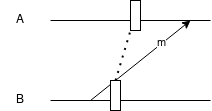
\includegraphics{fig/checkpoint_inconsistency.png}
    \caption{Operator B sends a message \emph{m} to operator A and both operators 
    committed a checkpoint of their internal state.}
    \label{fig:checkpoint_inconsistency}
\end{figure}

\subsubsection{Upstream backup}

\begin{figure}[!htbp]
    \centering
    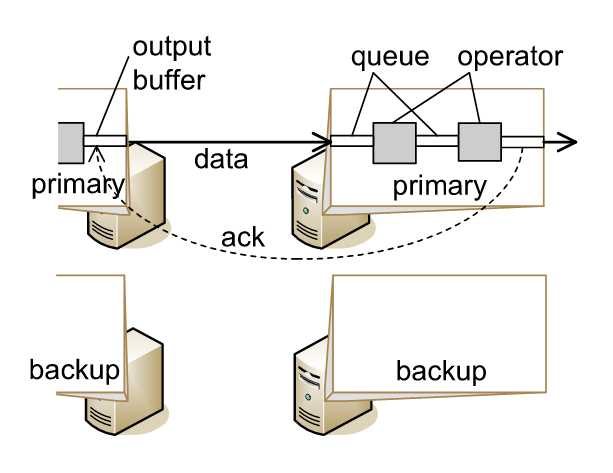
\includegraphics[width=0.5\textwidth]{fig/upstream.png}
    \caption{Upstream backup~\cite{upstream_backup}. }
    \label{fig:upstream}
    
\end{figure}


In this approach of fault tolerance, upstream operators 
will temporarily 
keep the tuples in their output buffer for subsequent operators. The tuples 
stay in the buffer until they are completely processed by the child operator. 
The buffer will then be cleared when the parent operator receives 
an acknowledgement from its children, as illustrated in the Figure~\ref{fig:upstream}. 

The drawback for this approach is that, the buffer might not be large enough to 
hold the records stored between the failure and the recovery event. Moreover, 
the whole system needs to be halted until the new operator catches back up to 
the state of the failed operator from the replayed records. 

\section{Data Stream processing}

Owing to the characteristics described in Section~\ref{sec:characteristics_data_stream}, 
processing data streams requires a different approach from that of a batch data processing engine.
Batch processing is defined as processing a small subset of the data simultaneously~\cite{batch_processing}. 
Originally, it is meant to tackle a particular characteristic of Big Data; the \textbf{volume}. The job 
could therefore last from several hours to days, depending on the volume of the data and the 
complexity of the operations~\cite{batch_duration}.
Consequently, batch processing engines do not need to take the continuous and 
timely nature of the data into account~\cite{flink}.

On the other hand, stream processing requires the notion of time and continuity of the data as 
specified earlier in Section~\ref{sec:characteristics_data_stream}. This brings several challenges 
that stream processing frameworks need to solve, resulting in a specialised architecture employed by the 
frameworks. In this section, we will summarise the general architecture and strategies to deal with the 
uncertainty of the order of items and the continuously processing of items in data streams. Different 
state of the art frameworks will also be briefly mentioned, to get the reader familiar with the 
frameworks. 

\newpage

\subsection{Lambda architecture}

As stated in the previous section, batch processing introduces long latency --- if a query 
is executed against a batch processing engine, it can take hours to return the results, which might be 
out of date once they are ready. To process the unbounded data stream with low latency and maximal accuracy,
one could combine the speed of stream processing with the accuracy of batch analysis. 


Lambda architecture~\cite{lambda_arch, lambda_arch_book, lambda_arc_bpost} introduced by Nathan Marz, is a 
design pattern to combine the high accuracy of batch analysis and the low latency of 
stream processing engines. It consists of three separate layers; a \textbf{batch} layer, 
a \textbf{speed} layer and a \textbf{serving} layer. 

To further complement the three layers, 
the data stream is also split into two different paths: 
\begin{itemize}
    \item A \textbf{cold} path --- data flowing in the cold path is not required to fulfil the low
        latency requirement. The \textbf{batch} layer is located along the cold path.   
    \item A \textbf{hot} path --- data along the hot path is constrained by the low latency requirement 
        and needs to be processed at high velocity. Therefore, it flows through the 
        \textbf{speed} layer.  
\end{itemize}

\begin{figure}[!htpb]
    \centering
    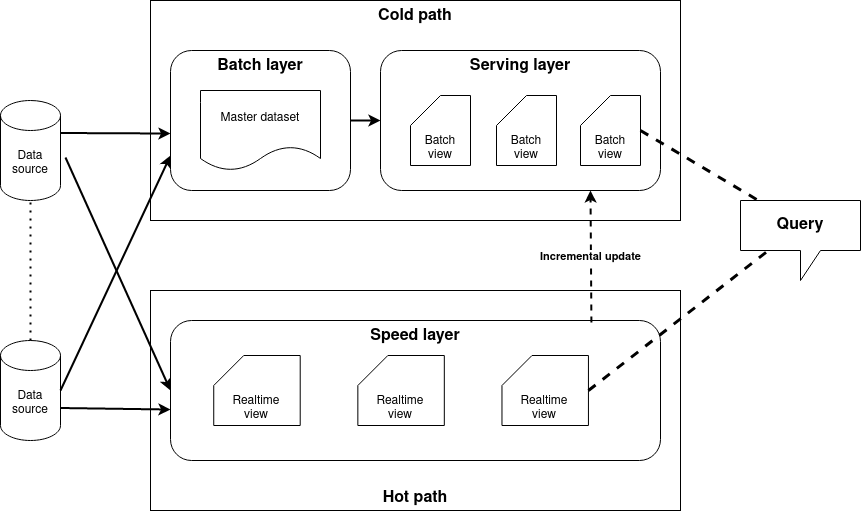
\includegraphics[width=\linewidth]{fig/lambda_arch.png}
    \caption{A general overview of the Lambda architecture. User queries are served from 
    the real-time views until the batch views are ready. Incremental updates could also be applied 
to the batch views in the \textbf{serving} layer by using the results from the \textbf{speed} layer.
~\cite{lambda_arch_book}}%
    \label{fig:lambda_arch}
\end{figure}

\subsubsection{The three layers}
The three layers serve to enhance the result of the users' queries by taking 
advantage of both the low latency of the \textbf{speed} layer and the accurate analysis of the \textbf{batch}
layer. 

\paragraph{Speed layer}%
\label{par:Speed layer}
The speed layer is responsible for processing the incoming data at high velocity and low latency. 
This layer focuses at low latency processing at the cost of a lower accuracy. The generated 
\textbf{realtime views}  could also be used to incrementally update the \textbf{batch views} since they 
are more recent due to low latency processing. Stream processing engines are employed in this 
layer. To ensure that the 
analysis is done on a subset of the whole streaming data, \textbf{windowing operators} are employed 
to restrict the stream processing to the elements contained within the \textbf{window}. For more information,
Chapter~\ref{chap:windows} will explore and elaborate the different \textbf{windows} that 
are commonly used in stream processing. 

\paragraph{Batch layer}%
\label{par:Batch layer}
The batch layer will store the incoming stream data in a master dataset. This master dataset is an immutable,
and append only dataset, to ensure that there is some notion of time or history of the data. Changes made to 
the previously stored data are re-appended to the dataset as a record with a new timestamp.  
This enables re-computation of the master dataset resulting in a new batch view as the dataset evolves over time. 
As the name suggests, batch processing engines are commonly deployed in the batch layer. For example, 
a MapReduce~\cite{mapreduce} framework like Apache Hadoop~\cite{hadoop} is commonly used in this 
layer for batch analysis. 


\paragraph{Serving layer}%
\label{par:Serving layer}

The serving layer receives the batch views from the batch layer and updates them as necessary. When a user 
queries the application, the serving layer will redirect the user to the real-time views if the 
requested data needs to be timely. Otherwise, the batch views will be returned to the user which are 
more accurate but less timely.  


\subsubsection{Summary}%
\label{ssub:Summary}

Separating the whole processing system into two separate components along 
the two different data paths, the \textbf{batch} layer on the \textbf{cold} path, and 
the \textbf{speed} layer on the \textbf{hot} path, introduces complexity in maintaining the business logic of the system.
If 
there is any change in the type of analysis done in one layer, the other layer needs to be updated 
with the corresponding batch analysis task. Therefore, there is unnecessary complexity in managing 
the system along the two dataflow paths. 
    

\subsection{Kappa architecture}%
\label{sub:Kappa architecture}
Proposed by Jay Kreps, Kappa architecture~\cite{kappa_architecture} is designed to replace the 
two processing systems layout of the Lambda architecture by combining batch and stream processing 
into one layer. Intuitively, stream processing is 
only meant to handle a very small subset of the whole data. However, if one were to be able 
to replay the historical data at high velocity, one could increase the parallelism of the streaming 
job and reprocess the whole historical data as a \emph{subset}. This results in an output accuracy similar
to that of the output from batch analysis. The Kappa architecture is based on this intuition.   

Instead of consuming the streaming data sources directly with the stream processing engine, 
the input data is first stored in a distributed data log system like Apache Kafka~\cite{kafka}. The data 
logs can be stored indefinitely or temporarily depending on the use case.
The stream processing layer has access to the data in two forms; 
a stream of events in real-time, or as a replay of historical data for batch analysis. 

\begin{figure}[!htbp]
    \centering
    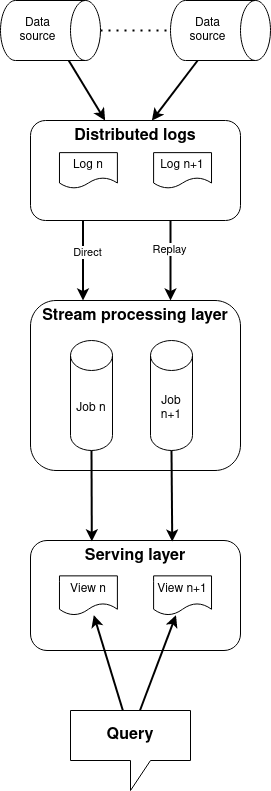
\includegraphics[width=0.4\linewidth]{fig/kappa_arch.png}
    \caption{An overview of the Kappa architecture. Here, job \emph{n+1} is re-processing using the replay 
    data from the unified data logs in parallel. Once it has caught up to the output of job \emph{n}, 
    job \emph{n} can be phased out and allow the latest job \emph{n+1} to take over.}
    \label{fig:kappa_arch}
\end{figure}


\subsubsection{Summary}%
Even though the Kappa architecture solves the problem of code redundancy and complexity of 
system management introduced in the 
Lambda architecture, it is not meant as a full replacement for the Lambda architecture. 
The Lambda architecture is useful in cases where a system needs to have two different algorithms for 
batch analysis and stream processing. For example, the batch layer could be responsible for training 
a machine learning model on the bounded dataset batches and improving the 
predictions, while the speed layer could deploy these models to provide real-time predictions. 


In this thesis, we are investigating the usage of dynamic windows in the context of stream processing 
non-heterogenoeus data to RDF data. 
Therefore, the Kappa architecture is the best candidate to deploy and test our 
hypotheses since we have no need for batch analysis in this thesis.  

\subsection{Out of order processing}%
\label{sub:Out of order processing}
Stream events can arrive out of order due to a myriad of reasons; network latencies, 
bad connections or a delay at one of the multiple sensors generating the events for 
the stream processing engine. As stated at the beginning of this chapter, stream 
processing engines should be aware of the timeliness of the data stream --- it needs 
to be able to deal with out-of-order events. 

To understand the strategy involved in the handling out-of-order events, 
two notions of \emph{time}~ need to be introduced~\cite{watermark_flink}:  

\begin{defn}[Processing time]
    Processing time refers to the time of the system on which the stream processing 
    engine is being executed. The system clock of the machine is therefore used 
    to mark the \emph{processing time}. 
\end{defn}
Marking events with processing time makes them 
susceptible to the speed and the order in which they arrive in the system. 
In a distributed environment, on which stream processing engines are often 
executed, processing time does not provide determinism. This is because 
reprocessing the same set of data stream will not lead to the same output, if 
the two execution are executed in sequence, since the processing time will be 
different, resulting in different watermarks. 


\begin{defn}[Event time]
    Event time is the time at which the events are generated at the source.
\end{defn}
For example, if user click events are being emitted at the
source, the \emph{event time} will be the time the user clicks on an object of 
interest. This timestamp is usually included in the record as they arrive 
in the stream processing engine. The engine could then extract these 
timestamp to use as \emph{event time}. 


\subsubsection{Watermarking}%
\label{ssub:Watermarking}

The two notions of \emph{time} are used in a strategy called \textbf{watermarking}. 
Watermarks are timestamp threshold used to deal with \emph{very late} events 
in the data stream. It specifies how long the stream processing engine 
waits for \emph{late events}. For example, if a watermark with timestamp 
20 arrives in the dataflow, the system could assume that all events 
with timestamp earlier than 20 already have arrived in the system. 

Just having these notions of time and watermarks is not enough to 
handle out-of-order events. The stream processing engine needs to be able to compare them to a subset of the 
incoming data. Windowing provides a grouped view of the infinite unbounded stream, 
enabling the engine to compare the subset of records for timeliness and out-of-order 
processing. A window can be \emph{time driven}, every $N$ seconds, or \emph{data driven}, 
every $N$ records. 
Suppose in Figure~\ref{fig:watermark}, a time window is applied on the stream that
stretches from watermark \emph{W(17)} until \emph{W(11)}. 
Once \emph{W(17)} arrives in the window, it knows that it contains or has 
processed all events earlier than timestamp 17 and later than timestamp of 11.  

However, it is possible for an event, later in the future, to arrive in the window 
with a timestamp earlier than 17. That event can be considered late as an outlier and 
be dealt with appropriately as defined by the developer. Different windows 
behave differently with the watermarking strategy. Chapter~\ref{chap:windows}
will dive deep into the workings of different windows and how windowing works in 
general. 


\begin{figure}[htpb]
    \centering
    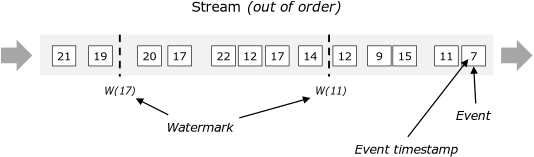
\includegraphics[width=0.8\linewidth]{fig/stream_watermark_out_of_order.png}
    \caption{Out of order events in a stream with watermarks~\cite{watermark_flink}.}
    \label{fig:watermark}
\end{figure}


\section{Frameworks}
\label{sec:frameworks}
There are state of the art stream processing frameworks widely employed across the 
different disciplines in the industry. These frameworks address the main challenges of 
Big Data stream processing, the three V's, differently with their own advantages and 
disadvantages.
In this section, we will elaborate 
on a few of these stream processing frameworks to identify the best characteristics of a 
stream processing engine and the different implementation to tackle the challenges by these 
frameworks.



\subsection{Apache Spark Streaming}%
\label{sub:Apache Spark}
Apache Spark~\footnote{Apache Spark: \url{https://spark.apache.org/}} is a batch 
processing framework developed to improve upon the existing implementations of the 
MapReduce paradigm. Instead working purely with a distributed file based system like 
Hadoop, Spark processes data in RAM with a read-only data structure called 
\emph{Resilient Distributed Dataset} also known as RDD. RDD is distributed over 
different machines in the cluster allowing parallel operations. Fault tolerance 
is also enabled through incremental bookkeeping of how RDD is built over time, allowing 
it to be rebuilt in case of failure.

These RDDs are the crucial building block to implement the stream processing engine 
based on Spark; Apache Spark Streaming~\cite{spark_streaming}. Spark Streaming structures
stream processing as a series of \emph{stateless, deterministic micro batch
computations} on small interval times~\cite{spark_streaming}. Discretizing the stream 
into micro batches frees up the stream processing engine from synchronization protocols 
and dependency of the data across time. Since the stream is modelled as \emph{micro} 
batches, the powerful recovery mechanisms and exactly-once delivery semantics of the traditional batch processing engines could
be applied. 
Furthermore, this seamless integration of RDDs, meant for batch analysis in 
streaming context, meant that Spark Streaming could utilize the Kappa architecture 
to maintain low latency stream processing. 

However, because the stream is discretized into micro batches, Apache Spark Streaming still has a 
higher latency when compared to systems processing individual records in the stream
such as Apache Flink and Apache Storm. 


\subsection{Apache Storm}%
\label{sub:Apache Storm}

Apache Storm~\footnote{Apache Storm: \url{https://storm.apache.org/}} is 
conceived by Nathan Marz, the mind behind the Lambda Architecture. In comparison to 
the micro batches structure of the stream in Spark Streaming, Storm's architecture 
consists of \emph{streams of records} flowing through
\emph{topologies}~\cite{storm_twitter}. This is a structure where operators are 
represented as \emph{nodes} and the data flow between these operators as \emph{edges} of 
a directed acyclic graph (DAG) as shown in Figure~\ref{fig:dag_topology}. 
The \emph{nodes} are further distinguished between 
two main functions; \emph{spouts} (data sources) and \emph{bolts} (computations).  
By processing the stream events as individual records, the latency is kept 
to a minimum in the \emph{bolts}. 

Furthermore, Storm provides at-least-once 
delivery semantics through the use of record-level acknowledgements. A randomly 
generated "id" is attached to each new record and an extra \emph{acker node} is attached 
to the execution graph. This \emph{acker node} is responsible for tracking the records, 
enabling at-least once delivery semantics. Storm could be upgraded to enable 
exactly-once semantics with the utilization of an API called
Trident~\footnote{Trident API: \url{https://storm.apache.org/releases/2.1.0/Trident-API-Overview.html}}. 
However, Storm would then structure the stream events as mini batches just like 
Spark Streaming, forfeiting the low latency processing. 

Due to its low-level definition of the \emph{bolts}, implementing computation tasks 
in Storm is non-trivial, and requires the implementation of one or more readers and 
collectors. This results in non-intuitive composition of the execution topology. 
Furthermore, Storm does not support 
batch processing, offering no options to extend the functionality of the stream 
processing application if batch processing support is required in the future. 


\begin{figure}[!htpb]
    \centering
    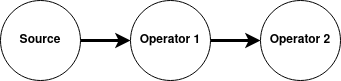
\includegraphics[width=0.5\linewidth]{fig/dag.png}
    \caption{A common stream processing topology representation as a DAG.} 
    \label{fig:dag_topology}
\end{figure}

\subsection{Apache Flink}%
\label{sub:Apache Flink}

Apache Flink~\cite{flink} aims to bridge the gap between batch and stream processing aspects of 
Big Data and combine them into one unified framework. Similar to Storm, 
Flink's execution topology is also internally represented as a DAG as shown 
in Figure~\ref{fig:dag_topology}. It also processes the incoming records as 
individual events to maintain low latency processing. Flink recognizes that
dedicated batch processing is still needed for applications where no efficient algorithms 
exist for performing the same analysis on streaming data. Therefore, Flink implements a 
specialized API for batch processing on top of its streaming processing engine.

Due to the focus on both batch and stream processing, Flink could fulfil the use cases for which 
Spark and Storm specializes in; batch processing and stream processing respectively. Furthermore, 
Flink provides exactly-once delivery semantics, overcoming the need to filter out duplicate 
results and calculation. This is achieved by implementing a variation of the \emph{Chandy-Lamport} algorithm
called \emph{Asynchronous Barrier Snapshotting} (ABS)~\cite{asynchronous_barrier}.
It is much more lightweight than Storm's record-level 
acknowledgements for both fault tolerance and exactly-once delivery semantics
due to the usage of in-stream barriers.  

Finally, Flink provides high-level APIs that make development easier for developers in 
the style of functional programming; an intuitive style for the use cases in the data analysis community. 
Windows are supported in Flink as an integral part of the engine with easy to use high-level APIs for 
commonly used windows (elaborated more in Chapter~\ref{chap:windows}).  
It also provides access to low-level APIs to implement highly customised windowing logic, without burdening 
the developers with the complexity of the internals of Flink. 
With the ease of development, the aforementioned low latency, and exactly-once delivery semantics, 
Flink is the best candidate to move forward with the implementation of dynamic windows for this thesis. 
